\chapter{Introduction}

Ship handling is the task of precisely controlling a seafaring vessel’s movement using its propulsion and navigation systems. Vessels move in a variety of marine environments. Starting from shallow waters of a harbor they often navigate vast seas to a port in another harbour across the ocean. Vessels also navigate inland waterways such as rivers, canals, backwaters and creeks. More recently, developments in offshore wind farming, the oil and gas industry have necessitated regular visits to offshore structures located on continental shelves for construction and maintenance activities. In handling a ship in such varied environments, a seafarer needs to take into account environmental forces such as wind, waves and current acting on the ship \parencite{wiki:seamanship}.

\todo{establish niche}
Navigation in marine environments as in aviation requires the navigator to assimilate information about various environmental factors that affect the task. The information is presented in various display panels placed around the navigator in the ship bridge. In 1955, the US Navy began researching head-up displays to reduce complication of aircraft instrumentation in an effort to make it easier for pilots to fly modern aircrafts. By 1970s, the use of HUDs for piloting was expanded beyond military aircraft to commercial aviation. Even though aviation and maritime navigation present similar challenges for a navigator, the use of head-up displays is not yet commonplace in the latter. 

The maritime sector is a niche market with a segmented market-space (many small and medium-sized companies), low R\&D intensity and, a conservative attitude towards innovation \parencite{von2014maritime}. Nevertheless, some research can be found on maritime applications of augmented reality. Some of them can be found in \cite{hugues2010experimental}, \cite{vasiljevic2011augmented} and, \cite{von2014maritime}. These applications have focused on augmenting the visual perception of users with real-time information; potentially helping them perform the job more efficiently. For example, overlaying the view from the bridge of a ship with route waypoints, distance to next waypoint, local hazards, and navigational aids such as buoys, lighthouses. 

However, there has been little research on the use of mixed reality technologies to create simulation environments for training purposes even though simulation is used extensively for ship operations training.

\section{Research Method}
Description of sce method goes here.


\section{Augmented Reality}
\label{sec:augreal}
Mixed reality refers to the merging of virtual and real worlds in which physical and digital objects co-exist and interact in real time. In the field of mixed reality, some distinctions have been made between various applications based on the amount of virtual content in the mix. A continuum has been drawn characterising different mixed reality environments as shown in figure \ref{fig:mixedrealitycontinuum}. Completely real and completely virtual environments bring up extreme ends of the continuum, with different levels of virtuality in between. 

\begin{figure}
	\centering
	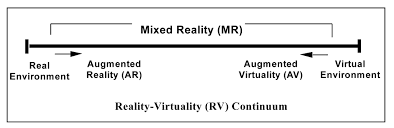
\includegraphics[width=\linewidth]{mixedrealitycontinuum}
	\caption{Mixed Reality Continuum (Source: \cite{milgram1995augmented})}
	\label{fig:mixedrealitycontinuum}
\end{figure}

Augmented reality has been defined by \textcite{azuma1997survey} as having the following three characteristics: 

\begin{enumerate}
	\item Combines real and virtual 
	\item Is interactive in real time
	\item Is registered in three dimensions
\end{enumerate} 

Virtual reality has been gaining popularity in the consumer market in recent years. It is a specific type of mixed reality featuring entirely digital visuals and virtual environments. No clear distinctions are made between points in the continuum. One particular construct, augmented reality, has been gaining popularity over the years. Augmented reality refers to systems that feature predominantly real environments whose perception maybe augmented with information not readily available to the user (figure \ref{fig:augreal} for example, shows a map overlay on top of the camera view of a street). Further, some factors have been identified that help distinguish between different mixed reality systems: extent of world knowledge (whether the augmentation takes place in a modeled world or not), reproduction fidelity (quality of display of the real/virtual objects) and extent of presence metaphor (extent to which user feels they are present in the displayed scene themselves). A detailed description of mixed reality displays and differences in their characteristics can be found in \cite{milgram1995augmented}. 

\begin{figure}
	\centering
	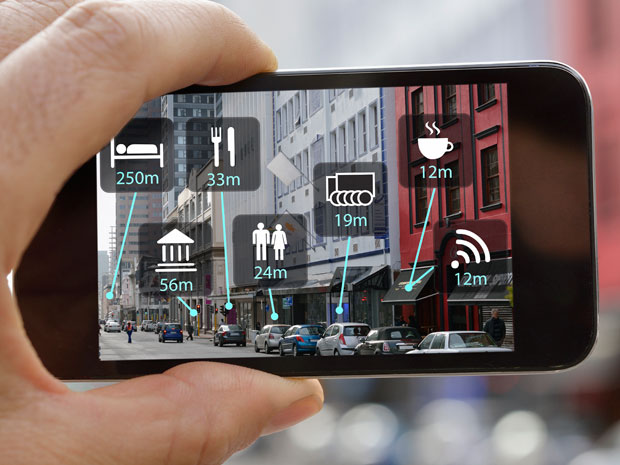
\includegraphics[width=\linewidth]{augreal}
	\caption{View of a street 'augmented' with information on places of interest}
	\label{fig:augreal}
\end{figure}
